%\chapter{Introduction to Linear Programming}
\chapter{Hamiltonian Graphs}
\paragraph{Motivation}
We are interested in the Eulerian graph, i.e., 
whether there exists a closed trail (that travels each edge once and only once), for a connected graph.
There is a simple necessary and sufficient condition for a graph to be Eulerian: \emph{every vertex has even degree}.
Similarly, is there a cycle that includes every vertex once and only once, for a connected graph?

\begin{definition}[Hamiltionian]
\begin{enumerate}
\item
A \emph{Hamiltonian cycle} in a graph is a \emph{cycle} that includes every vertex (once and only once).
\item
A graph is \emph{Hamiltonian} if it contains a Hamiltonian cycle.
\item
A non-Hamiltonian graph is \emph{semi-Hamiltonian} if there exist a \emph{path} through every vertex.
\end{enumerate}
\end{definition}

However, not all graphs are \emph{Hamitonian}. We are studying necessary or sufficient conditions for a graph to be Hamiltonian.

\section{Necessary Conditions}

\begin{theorem}
If $G$ is Hamitonian, then for each non-empty set $S\subseteq V$, the graph $G-S$ has at most $|S|$ componenets.
\end{theorem}
As a result, \emph{every Hamitonian graph must be $2$-connected}.
\begin{proof}
Consider a Hamiltionian cycle in $G$, which must pass through all vertices including both $G-S$ and $S$.
Each time when leaving a component of $G-S$, it must go next to a vertex in $S$, and must be a distinct vertex in $S$.
Therefore, the number of components of $G-S$ cannot be more than the number of vertices in $S$.
\end{proof}
\begin{remark}
However, the converse may not be necessarily true. Consider the counter-example
\begin{figure}[H]
\centering
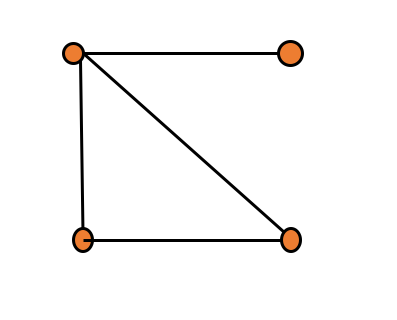
\includegraphics[width=0.7\textwidth]{Third_lecture/p_2}
\end{figure}
\end{remark}
\section{Sufficient Conditions}
Most sufficient conditions are of the form:
\emph{If the graph has enough edges, then it is Hamiltonian}.

\begin{theorem}[Ore’s theorem]
If $G$ is a simple graph with $n\ge 3$ vertices, and if 
\[
\text{deg}(v)+\text{deg}(w)\ge n,
\]
for each pair of non-adjacent vertices $v$ and $w$, then $G$ is Hamitonian.
\end{theorem}
\begin{proof}
Suppose on the contrary that $G$ is not, and w.l.o.g., $G$ is maximal.
Thus there must be a path $v_1\to v_2\to\cdots\to v_n$ passing through each vertex but $v_1$ and $v_n$ are non-adjacent.
Therefore, $\text{deg}(v_1)+\text{deg}(v_n)\ge n$, i.e., there must be a vertex $v_i$ adjacent to $v_1$ with the property that $v_{i-1}$ is adjacent to $v_n$, which leads to a Hamitonian cycle:
\[
v_1\to \cdots\to v_{i-1}\to v_n\to v_{n-1}\to v_{n-2}\to\cdots\to v_i\to v_1
\]
\end{proof}

\begin{corollary}
If $G$ is a simple graph with $n\ge 3$ vertices, and $\text{deg}(v)\ge\frac{1}{2}n$ for each vertex $v$, then $G$ is Hamiltionian.
\end{corollary}

\begin{theorem}
If $G$ is a simple graph with $n\ge 3$ vertices, and if $G$ has at least $(n-1)(n-2)/2+2$ edges, then $G$ is Hamitionian.
\end{theorem}
\begin{proof}
\begin{enumerate}
\item
If every vertex is adjacent to every other vertex, then $G$ is complete, and therefore Hamitonian
\item
Otherwise, let $v$ and $w$ be two non-adjacent vertices, and $H=G-\{v,w\}$ contains $(n-2)$ vertices, with maximum number of edges $(n-2)(n-3)/2$.
There exists at least $(n-1)(n-2)/2+2 - (n-2)(n-3)/2=n$ vertices incident to either $v$ or $w$. Therefore, $\text{deg}(v)+\text{deg}(w)\ge n$. By applying Ore's theorem, $G$ must be Hamitonian. 
\end{enumerate}
\end{proof}


\begin{theorem}\label{The:3:5}
Let $G=(V_1\cup V_2)$ be a bipartite graph.
If $G$ is Hamitonian, then $|V_1|=|V_2|$.

If $G$ is semi-Hamitonian, then $|V_1|$ and $|V_2|$ differ by at most 1.
\end{theorem}
\begin{proof}
Consider the Hamitonian cycle.
\end{proof}

\begin{corollary}
The converse of Theorem~(\ref{The:3:5}) also holds if $G$ is a \emph{complete} bipartite graph with at least 3 vertices.
\end{corollary}
\begin{proof}
Construct the Hamitonian cycle.
\end{proof}

\begin{definition}[Hamiltonian Closure]
The \emph{Hamiltonian closure} of a graph $G=(V,E)$ is the graph $C(G)$ obtained from $G$ by iteratively adding edges joining pairs of \emph{non-adjacent} vertices whose degree sum is at least $|V|$, until no such pair remains.

If $G=C(G)$, then we say $G$ is closed.
\end{definition}
The closure does not depend on the sequence by which the edges are added.

\begin{lemma}
The \emph{Hamitonian closure} of a graph $G=(V,E)$ is well-defined.
\end{lemma}
\begin{proof}
Suppose we add sequence of edges $\{e_1,\dots,e_f\}$ to form $G_1$ and $\{f_1,\dots,f_s\}$ to form $G_2$.

Note that a pair of vertices $(u,v)$ are added iff theya are non-adjacent and the sum of degree is at least $n=|V|$.
Thus by definition, $f_1$ is addable to $G$, and must be added at some point in the first sequence, i.e., $f_1\in G_1$.
Inductively, $f_1,f_2,\dots,f_s\in E(G_1)$, which implies $E(G_2)\subseteq E(G_1)$.
Similarly, $E(G_1)\subseteq E(G_2)$.
\end{proof}


\begin{theorem}[Bondy-Chvatal]
A simple graph $G$ is Hamitionian if and only if its closure $C(G)$ is Hamitionian
\end{theorem}
\begin{proof}
Clearly, if $G$ is Hamitonian, so is $C(G)$. Conversely, let $\{G_0:=G,G_1,\dots,C(G)\}$ be a sequence of graphs where each $G_i$ is formed by performing a single closure step to $G_{i-1}.$
Let $k$ be the minimal value such that $G_k$ is Hamiltonian.
Let $(w,u)$ be the edge added to form $G_k$ from $G_{j-1}$ and let $C$ be a Hamiltionian cycle in $G_k$.
Therefore, $C$ must contain the edge $(w,u)$, and suppose it is of the form
\[
u:=v_1\to\cdots\to v_n=w\to u.
\]
Now we argue that $G_{k-1}$ is Hamiltonian.
Since there are $n$ edges incident to either $u$ or $v$, there exists a vertex $v_i$ incident to $u$ such that $v_{i-1}$ is incident to $w$ in $G_{k-1}$, which leads to a Hamitonian cycle in $G_{k-1}$:
\[
u=v_1\to v_i\to v_{i+1}\to\cdots\to v_n=w\to v_{i-1}\to v_{i-2}\to\cdots\to v_2\to v_1=u
\]
\end{proof}

\begin{theorem}[Chvatal]
Let $G$ be a simple graph on $n\ge3$ vertices with degrees $d_1\le d_2\le\cdots\le d_n$.
If for all $i<n/2$,
either $d_i>i$ or $d_{n-i}\ge n-i$, then $G$ is Hamiltonian.
\end{theorem}
\begin{proof}
It suffices to consider the case where $G$ is closed.
Suppose on the contrary that $G=C(G)$ is non-Hamitonian, which is not complete.
Among all pairs of non-adjacent vertices, let $(u,v)$ be the pair with maximum degree sum, w.l.o.g., $\text{deg}(u)\le\text{deg}(v)$.
Since $G$ is closed, we have $\text{deg}(u)+\text{deg}(v)<n$, i.e., $\text{deg}(u)<n/2$.
Suppose that $\text{deg}(u)=k$, then every other vertex in $V$ not adjacent to $v$ must have degree no larger than $\text{deg}(u)=k$; there are $n-1-\deg(v)$ such vertices.
Note that $\text{deg}(u)+\text{deg}(v)\le n-1$ implies that $n-1-\deg(v)\ge\text{deg}(u)=k$.
Therefore, we have found $k$ vertices of degree at most $k$.

Similarly, every vertex that is not adjacent to $u$ has degree at most $\text{deg}(v)$.
By assumption, $\text{deg}(v)<n-k$.
There are $(n-1)-\text{deg}(u)$ such vertices.
Also, $u$ it self has the degree no larger than $\text{deg}(v)$, thus there are $n-k$ vertices with degree smaller than $n-k$.
\end{proof}

Consider for some sequence $(d_1,\dots,d_n)$ we have $d_h\le h$ and $d_{n-h}\le n-h-1$ for some $0<h<n/2$. Now we want to construct a graph with this degree sequence that is non-Hamitonian.

Consider one possible example:
\[
(\underbrace{h,\dots,h}_{\text{$h$ times}},
\underbrace{n-h-1,\dots,n-h-1}_{\text{$n-2h$ times}},
\underbrace{n-1,\dots,n-1}_{\text{$h$ times}},
)
\]
The graph has two components: a complete bipartite graph $K_{hh}$ with $V_1=\{v_1,\dots,v_h\}$ and $V_2=\{v_{n-h+1},\dots,v_n\}$ and a complete graph $K_{n-h}$ with $V=\{v_{h+1},\dots,v_n\}$.

\begin{definition}[Hamiltonian for Directed Graph]
Consider a \emph{directed} graph $D$. We say $D$ is \emph{Hamiltonian} if there is a directed cycle that includes every vertex of $D$.

A non-Hamiltonian digraph that contains a directed path through every vertex is semi-Hamiltonian.
\end{definition}

We are considering the necessary and sufficient conditions for a digraph to be Hamiltonian; and are there some special types of graphs more likely to be Hamiltonian?

\begin{definition}[Tournament]
A directed graph $D$ is a \emph{tournament}
if there is exactly one arc between every pair of vertices.
In other words, a tournament is an orientation of a complete simple graph.
\end{definition}

\begin{theorem}[Redei]
Every non-Hamiltonian tournament is semi-Hamiltonian, i.e., 
every tournament contains a Hamiltonian path
\end{theorem}
\begin{proof}
We show this result by induction on $|V|=n$.
Suppose the tournament $T-v$ contains a Hamitonian path, say $v_1\to\cdots\to v_{n-1}$, and show that $T$ has a Hamitonian path.
Consider three cases:
\begin{enumerate}
\item
There is an arc $(v,v_1)\in T$
\item
There is an arc $(v_{n-1},v)\in T$
\item
There is no arc for $(v,v_1)$ and $(v_{n-1},v)$
\end{enumerate}
In previous two cases, the result is trivial.
In the third case, define $i$ to be the smallest index such that $(v,v_i)$ is an arc in $T$.
Therefore, we construct a Hamitonian path:
\[
v_1\to v_2\to\cdots\to v_{i-1}\to v\to v_i\to v_{i+1}\to\cdots\to v_{n-1}
\]
\end{proof}


\begin{theorem}[Camion]
Every strongly connected tournament is Hamitonian.
\end{theorem}
\begin{proof}
For a strongly connected tournament $T$, it must have at least 3 vertices.
We will show that a tournament with $|V|=n$ contains cycles of length $3,4,\dots,n$ by induction.
\begin{enumerate}
\item
Base Case:
Consider any vertex $v$ in $T$. Since $T$ is strongly connected, there must be at least one vertex incident to $v$ and at least one vertex incident from $v$.
Let $V_{\text{in}}$ be the set of vertices incident to $v$, $V_{\text{out}}$ the set of vertices incident from $v$.
Since $T$ is strongly connected, there must be an arc $(v_o,v_i)\in V_{\text{in}}\times V_{\text{out}}$, and therefore a 3-cycle exists.
\item
It remains to show that if there is a cycle $C$ of length $k$, then there is also a cycle of length $k+1$.
Suppose there is a vertex $c$ not in the cycle such that 
there exists arcs incident to $c$ from some vertices in $C$, and arcs 
incident from $c$ to some vertices in $C$.
Thus there must be an arc $(u,v)$ in $C$ such that $T$ contains arcs $(u,c)$ and $(c,v)$. Thus we have a $(k+1)$-cycle.
\item
If no such vertex exists, then for each vertex $w$ not in the cycle, its arcs that are joined to vertices in the cycle are
either all incident from $w$,
or all incident to $w$.
Let $A$ and $B$ be the two (disjoint) sets of vertices with such properties.
Since $T$ is strongly connected, neither $A$ nor $B$ can be empty.
There must exist an arc from some vertex $b\in B$ to some vertex $a\in A$.
Therefore, we can replace two consecutive arcs in the $k$-cycle, say $(u,c)$ and $(c,v)$ by the arcs $(u,b),(b,a),(a,v)$ to get a $(k+1)$-cycle.
\end{enumerate}
\end{proof}

\begin{theorem}
Let $D$ be a strongly connected digraph with $n$ vertices.
If $\text{outdeg}(v)\ge n/2$ and $\text{indeg}(v)\ge n/2$ for every vertex $v$, then $D$ is Hamitonian.
\end{theorem}

\paragraph{The Travelling Salesman Problem}
Given the distance between each pair of cities (on a given list), we want to find a Hamiltonian cycle ( that visits all the cities on the list and return to his starting point), with mimimum distance.
How many Hamiltonian cycles in a complete graph? $\frac{(n-1)!}{2}!$
























